\documentclass[11pt,a4paper]{article}

\usepackage[margin=2cm]{geometry}
\usepackage[T1]{fontenc}
\usepackage[utf8]{inputenc}
\usepackage{lmodern}
\usepackage{xcolor}
\usepackage{tikz}
\usetikzlibrary{arrows.meta, positioning, shapes.geometric}
\usepackage{caption}

\pagestyle{empty}
\setlength{\parindent}{0pt}

\definecolor{fdBlue}{HTML}{284B63}
\definecolor{fdLight}{HTML}{F7F4EA}
\definecolor{fdGray}{HTML}{EEF2F4}
\definecolor{fdSoft}{HTML}{D9E4EC}

\tikzset{
  line/.style={-{Latex[length=3mm,width=2mm]}, thick, draw=fdBlue},
  startstop/.style={
    ellipse,
    draw=fdBlue,
    very thick,
    fill=fdSoft,
    minimum width=3.8cm,
    minimum height=1cm,
    align=center,
    font=\small\bfseries
  },
  process/.style={
    rectangle,
    rounded corners=3pt,
    draw=fdBlue,
    very thick,
    fill=fdLight,
    text width=4.2cm,
    minimum height=1.15cm,
    align=center,
    font=\small
  },
  decision/.style={
    diamond,
    aspect=2.0,
    draw=fdBlue,
    very thick,
    fill=fdGray,
    text width=3.0cm,
    align=center,
    inner sep=2pt,
    font=\small
  },
  output/.style={
    trapezium,
    trapezium left angle=75,
    trapezium right angle=105,
    draw=fdBlue,
    very thick,
    fill=white,
    text width=4.0cm,
    minimum height=1.1cm,
    align=center,
    font=\small
  }
}

\begin{document}

{\LARGE \textbf{Diagrama de flujo general - FincaDiag Modular}}\\[0.3cm]
Version intermedia del flujo principal del instrumento de apoyo tecnico-forense.

\begin{figure}[h!]
\centering
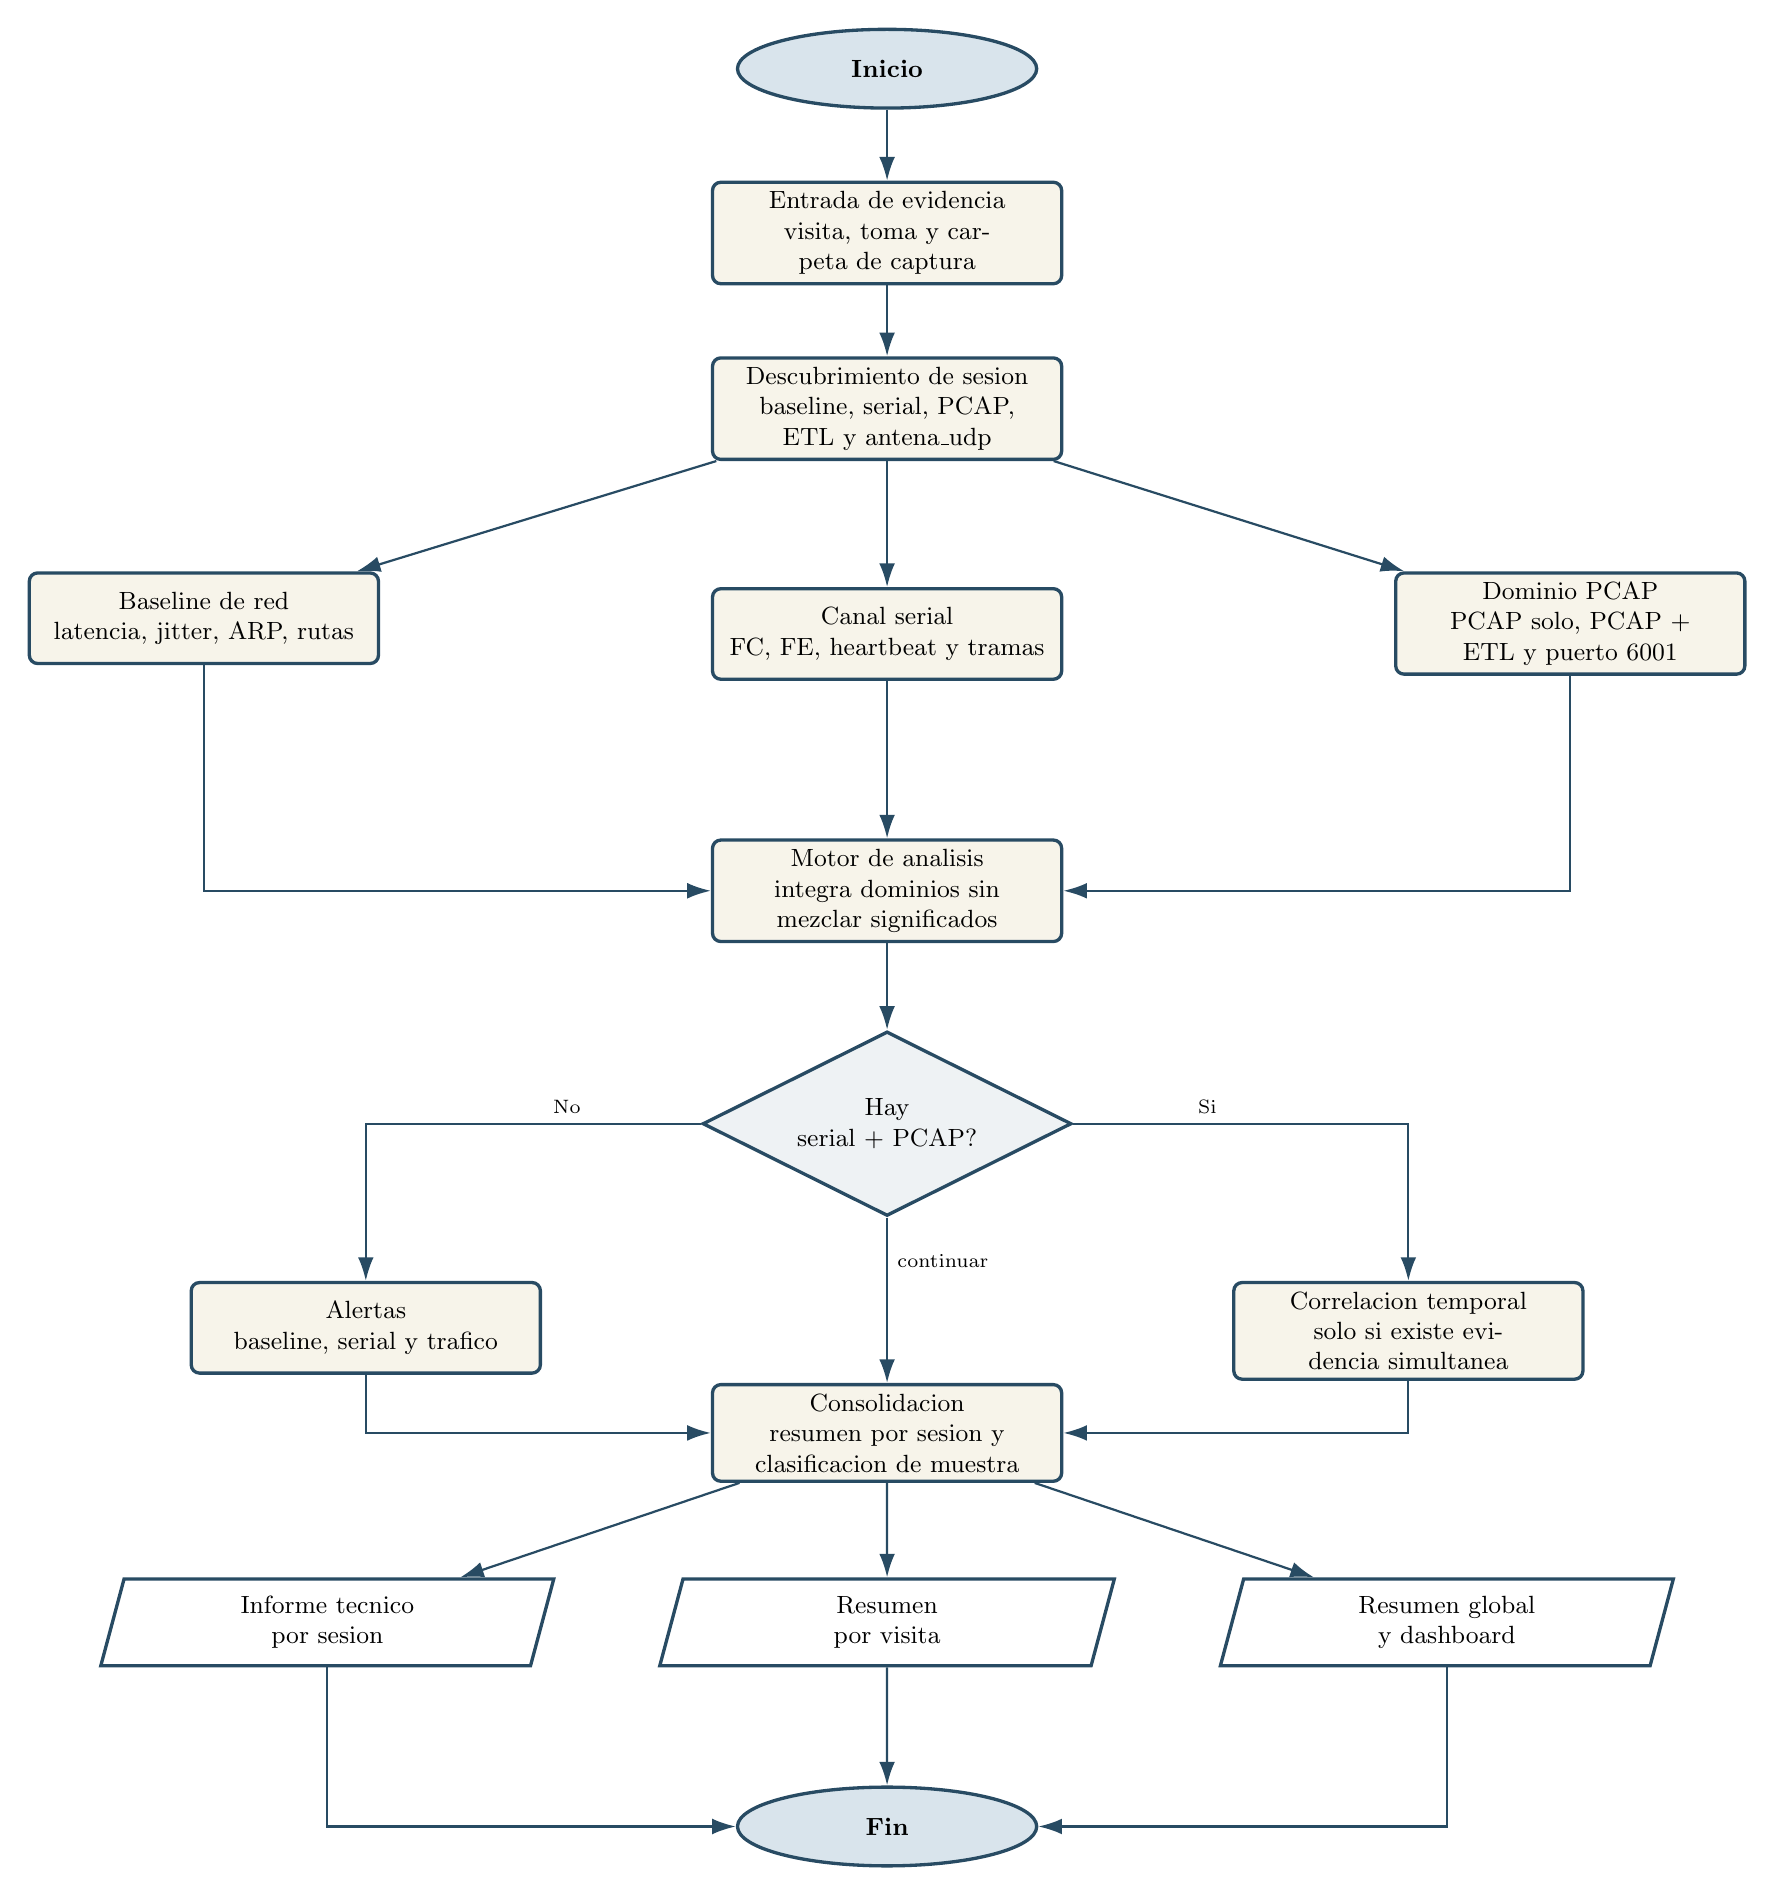
\begin{tikzpicture}[node distance=0.9cm and 1.2cm]

\node[startstop] (start) {Inicio};
\node[process, below=of start] (input) {Entrada de evidencia\\ visita, toma y carpeta de captura};
\node[process, below=of input] (discover) {Descubrimiento de sesion\\ baseline, serial, PCAP, ETL y antena\_udp};

\node[process, below left=1.4cm and 4.2cm of discover] (base) {Baseline de red\\ latencia, jitter, ARP, rutas};
\node[process, below=1.6cm of discover] (serial) {Canal serial\\ FC, FE, heartbeat y tramas};
\node[process, below right=1.4cm and 4.2cm of discover] (pcap) {Dominio PCAP\\ PCAP solo, PCAP + ETL y puerto 6001};

\node[process, below=2.0cm of serial] (engine) {Motor de analisis\\ integra dominios sin mezclar significados};
\node[decision, below=1.1cm of engine] (corr) {Hay\\ serial + PCAP?};
\node[process, below left=1.4cm and 3.2cm of corr] (alerts) {Alertas\\ baseline, serial y trafico};
\node[process, below right=1.4cm and 3.2cm of corr] (correlation) {Correlacion temporal\\ solo si existe evidencia simultanea};
\node[process, below=2.1cm of corr] (summary) {Consolidacion\\ resumen por sesion y clasificacion de muestra};

\node[output, below left=1.2cm and 4.3cm of summary] (hourly) {Informe tecnico\\ por sesion};
\node[output, below=1.2cm of summary] (visit) {Resumen\\ por visita};
\node[output, below right=1.2cm and 4.3cm of summary] (global) {Resumen global\\ y dashboard};
\node[startstop, below=1.5cm of visit] (end) {Fin};

\draw[line] (start) -- (input);
\draw[line] (input) -- (discover);

\draw[line] (discover) -- (base);
\draw[line] (discover) -- (serial);
\draw[line] (discover) -- (pcap);

\draw[line] (base) |- (engine);
\draw[line] (serial) -- (engine);
\draw[line] (pcap) |- (engine);

\draw[line] (engine) -- (corr);
\draw[line] (corr.west) -| node[pos=0.2, above, font=\scriptsize] {No} (alerts.north);
\draw[line] (corr.east) -| node[pos=0.2, above, font=\scriptsize] {Si} (correlation.north);

\draw[line] (alerts.south) |- (summary.west);
\draw[line] (correlation.south) |- (summary.east);
\draw[line] (corr.south) -- ++(0,-0.55) -| node[pos=0.18, right, font=\scriptsize] {continuar} (summary.north);

\draw[line] (summary) -- (hourly);
\draw[line] (summary) -- (visit);
\draw[line] (summary) -- (global);

\draw[line] (hourly.south) |- (end.west);
\draw[line] (visit) -- (end);
\draw[line] (global.south) |- (end.east);

\end{tikzpicture}
\caption*{Flujo general balanceado del procesamiento, analisis y consolidacion de evidencia.}
\end{figure}

\end{document}
